% Source: Code/ML_overlay/ir_rgb_registration/paper/ml_overlay_report_materials/ir_rgb_registration_report/figures/fig_synthetic_deformation_pipeline.tex
\documentclass[tikz,border=10pt]{standalone}
\usepackage{tikz}
\usetikzlibrary{shapes.geometric, arrows.meta, positioning, fit, calc}

\definecolor{Garnet}{RGB}{115, 0, 10}
\definecolor{Rose}{RGB}{204, 46, 64}
\definecolor{Atlantic}{RGB}{70, 106, 159}
\definecolor{Congaree}{RGB}{31, 65, 77}
\definecolor{Black90}{RGB}{54, 54, 54}
\definecolor{Black70}{RGB}{92, 92, 92}
\definecolor{Black30}{RGB}{199, 199, 199}

\tikzstyle{process} = [rectangle, minimum width=3cm, minimum height=1cm, text centered, draw=Garnet, fill=white, line width=1.2pt, font=\small]
\tikzstyle{arrow} = [-{Stealth[length=3mm]}, line width=1.5pt, Garnet]

\begin{document}
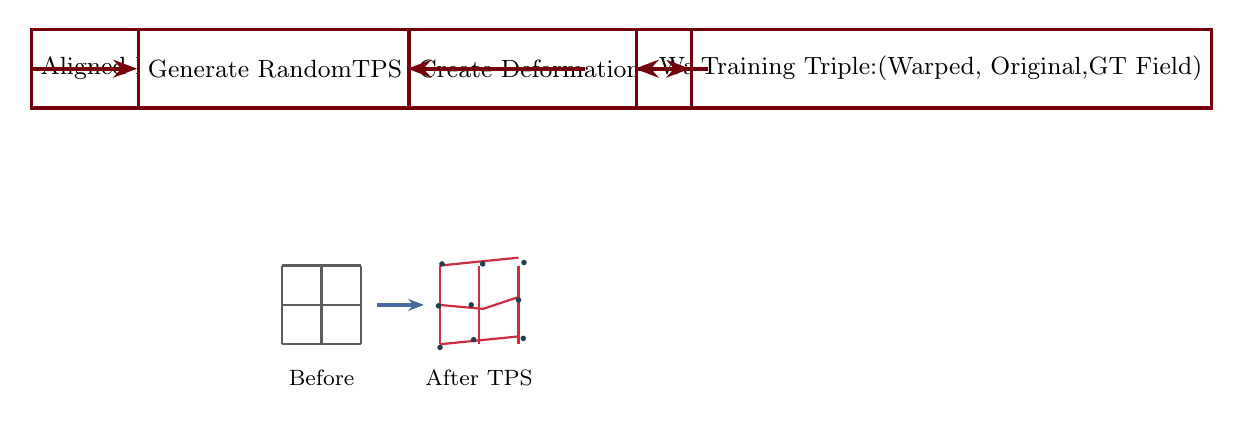
\begin{tikzpicture}[node distance=2.5cm]

% Main process boxes
\node (input) [process] {Aligned IR/RGB Pair};
\node (generate) [process, right of=input] {Generate Random\\TPS Control Points};
\node (field) [process, right of=generate] {Create Deformation\\Field};
\node (warp) [process, right of=field] {Warp One Image};
\node (output) [process, right of=warp] {Training Triple:\\(Warped, Original,\\GT Field)};

% Arrows
\draw [arrow] (input) -- (generate);
\draw [arrow] (generate) -- (field);
\draw [arrow] (field) -- (warp);
\draw [arrow] (warp) -- (output);

% Example grid deformation at TPS step
\begin{scope}[shift={($(generate)+(0,-2.5)$)}]
    % Original grid
    \draw[Black70, line width=0.8pt] (-1,-1) grid[step=0.5] (0,0);
    \node[below, font=\footnotesize] at (-0.5,-1.2) {Before};

    % Arrow
    \draw[-{Stealth[length=2mm]}, Atlantic, line width=1.2pt] (0.2,-0.5) -- (0.8,-0.5);

    % Deformed grid
    \begin{scope}[shift={(2,0)}]
        \draw[Rose, line width=0.8pt]
            (-1,-1) -- (-0.5,-0.95) -- (0,-0.9)
            (-1,-0.5) -- (-0.45,-0.55) -- (0,-0.4)
            (-1,0) -- (-0.5,0.05) -- (0,0.1);
        \draw[Rose, line width=0.8pt]
            (-1,-1) -- (-1,-0.5) -- (-1,0)
            (-0.5,-1) -- (-0.5,-0.5) -- (-0.5,0)
            (0,-1) -- (0,-0.5) -- (0,0);
        \foreach \i in {-1,-0.5,0}
            \foreach \j in {-1,-0.5,0}
                \fill[Congaree] (\i+0.1*rand,\j+0.1*rand) circle (1pt);
        \node[below, font=\footnotesize] at (-0.5,-1.2) {After TPS};
    \end{scope}
\end{scope}

\end{tikzpicture}
\end{document}
